% ============================================================
%  The European AI Summer Research
%  Paper template (recommended, optional)
%
%  HOW TO USE
%  ----------
%  1. Open this folder on Overleaf (overleaf.com) or compile
%     locally with pdflatex. Keep easrp2026.sty in the same folder.
%  2. Write your paper in the marked sections below.
%  3. Keep it ANONYMOUS: no names, no affiliations, no
%     identifying acknowledgements. See README.txt.
%  4. Compile to PDF and submit the PDF.
%
%  PAGE LIMIT: up to 8 pages of main text (11pt, A4).
%  References and any appendix do NOT count toward this limit.
%
%  When your paper is ACCEPTED, change the line
%      \usepackage{easrp2026}
%  to
%      \usepackage[accepted]{easrp2026}
%  and fill in \easrpauthor / \easrpaffiliation below to show
%  your name on the final version.
% ============================================================

\documentclass[11pt,a4paper]{article}

\usepackage{graphicx}             % for inserting images
% \usepackage{easrp2026}            % anonymous submission
\usepackage[accepted]{easrp2026}  % camera-ready (reveals authors)

% --- Author details: used only in the accepted version -------
% Leave these here; they are ignored while in anonymous mode.
\easrpauthor{Oleh Kovalyshyn, Yevhenii Zasko, Volodymyr Sydorskyi}
\easrpaffiliation{Kyiv School of Economics, Kyiv, Ukraine}

\easrptitle{Your paper title here}

\begin{document}

\maketitle

% Delete this note in your final paper.
\begin{center}
\fbox{\parbox{0.9\linewidth}{\small\itshape
Formatting: up to 8 pages of main text at 11pt on A4; references
and any appendix do not count toward the limit. Keep the
submission anonymous (no names, affiliations, or identifying
acknowledgements).}}
\end{center}

\begin{abstract}
Write a short abstract here, roughly 150--250 words: the
problem, your approach, and your main result, in plain
language. Do not include anything that identifies you or your
institution.
\end{abstract}

\section{Introduction}
% Introduce the problem and why it matters, and state your
% contribution clearly. Write in an anonymous style: refer to
% your own prior work in the third person (for example,
% ``Smith (2024) showed\ldots'') rather than ``our previous
% work''.

Contribution:
\begin{itemize}
    \item Enhance Suger ONE model with Jepa embedding to improve overall accuracy and adaptation to new patients. TODO: compare with fine-tune Suger One. Loss on spikes and reductions, unweighted patient loss
    \item Explore Standalone Glucose Jepa capabalilities, in terms of incapsulation of patient infromation (glucose specific). TODO: Retrain Australian Jepa on our train. 
\end{itemize}

\section{Related work}
Situate your work among existing research: summarise what has
been done, identify what remains open, and make clear how your
contribution differs. Cite credible, verifiable sources, and
prefer peer-reviewed papers where they exist. Preprints,
technical reports, datasets, theses, and software may be cited
when they are the appropriate source (as is common in machine
learning); avoid relying on non-authoritative web content such
as blog posts.

The accompanying bibliography file includes examples of several
reference types: a journal article \cite{lecun2015deep}, a
conference paper \cite{vaswani2017attention}, a book
\cite{russell2020aima}, a book chapter \cite{rumelhart1986learning},
a technical report \cite{krizhevsky2009cifar}, a thesis
\cite{sutton1984thesis}, a preprint \cite{devlin2018bert}, and a
web resource \cite{turing1950webexample}.

This template uses \texttt{natbib}, which offers several citation
commands. Use \verb|\citet| for a textual citation that reads as
part of the sentence: \citet{vaswani2017attention} introduced the
Transformer. Use \verb|\citep| for a parenthetical citation: the
Transformer dispenses with recurrence \citep{vaswani2017attention}.
The starred forms \verb|\citet*| and \verb|\citep*| list every
author rather than abbreviating with ``et al.'':
\citep*{vaswani2017attention}. You can also cite just the year with
\verb|\citeyear| \citeyear{lecun2015deep}, just the authors with
\verb|\citeauthor| \citeauthor{lecun2015deep}, or give multiple
references at once \citep{lecun2015deep, devlin2018bert}.

\section{Method}
\subsection{Proposed Approach}
\subsection{SugarOne Integration}

The pre-trained JEPA encoder was integrated into the SugarOne model as an additional covariate branch, following the same general design used for bolus, basal, and carbohydrate inputs. The resulting JEPA embeddings were layer-normalized and projected from 96 to 32 dimensions before being passed to the multi-head attention block (Figure~\ref{fig}).

\begin{figure}[ht]
\centering
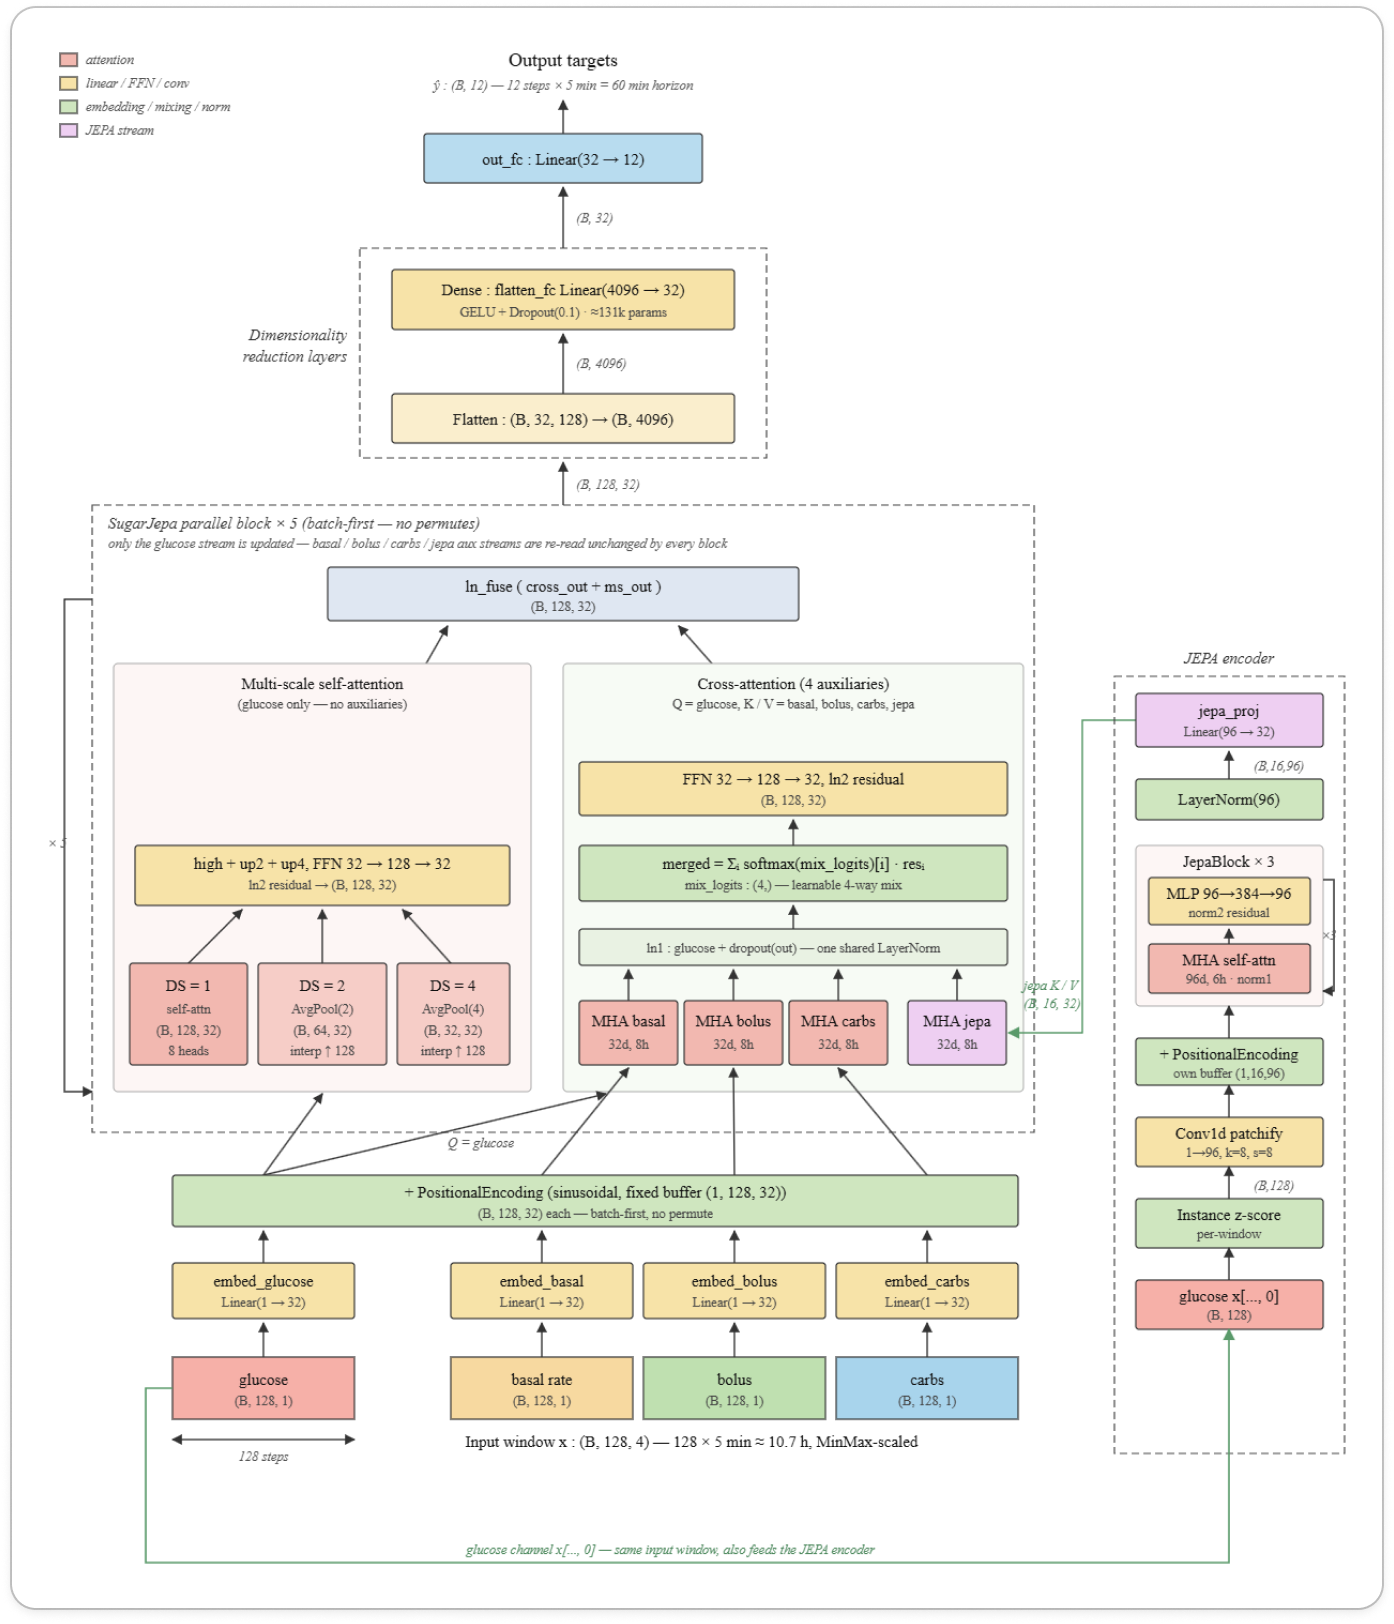
\includegraphics[width=0.8\textwidth]{sugar_jepa.png}
\caption{SugarJEPA architecture. SugarOne is augmented with an additional JEPA-based auxiliary branch.}
\label{fig}
\end{figure}

When the JEPA encoder required an input sequence of $m$ time points and SugarOne required only $n$ time points, with $m > n$, training windows were constructed to contain $m$ points. The full $m$-point sequence was passed to the JEPA encoder, while only the final $n$ points were provided to the main SugarOne branches.

We have shown that, in addition to improving overall predictive performance, JEPA provides SugarOne with strong zero-shot personalization capabilities, even outperforming SugarOne models fine-tuned for individual patients, as shown in Table~\ref{tab:sugar-jepa-finetuning}.


\subsection{JEPA as Patient Embedding}

One of the main practical challenges in glucose prediction is adaptation to an individual patient. Typically, such adaptation is performed through model fine-tuning, which requires accumulating a sufficient patient-specific dataset. During this data collection period, a personalized model cannot yet be deployed.

We hypothesize that JEPA representations can serve as patient embeddings, capturing sufficient patient-specific information to enable the SugarOne + JEPA model to operate in a zero-shot personalization setting. This approach still requires an initial observation period to produce a representative JEPA embedding; however, this period is typically substantially shorter than the time required to accumulate a dataset suitable for fine-tuning.

We compared SugarOne + JEPA against the standalone SugarOne model, with particular focus on patient-specific fine-tuning and zero-shot prediction (Table~\ref{tab:sugar-jepa-finetuning}). We found that SugarOne augmented with a JEPA embedding computed from only one day of patient data outperformed the standalone SugarOne model fine-tuned on 30 days of patient-specific data.

Additionally we trained a dense classification head on top of the frozen pre-trained JEPA encoder using a patient identification task. Depending on the JEPA input sequence length, the resulting patient recognition accuracy ranged from 10\% to 68\%. These results indicate that the learned JEPA representations contain substantial patient-specific information and provide evidence supporting their use as patient embeddings for zero-shot personalized glucose prediction.

\subsubsection{Additional Regularization}

Our JEPA encoder is based on the CGM-JEPA approach \cite{muhammad2026cgm}. In addition to the original Exponential Moving Average (EMA) regularization, we have added a variance regularization term inspired by VICReg \cite{vicreg}:

$$
L =
\underbrace{
\operatorname{SmoothL1}(\hat{z},z)
}_{\text{prediction loss}}
+
\lambda
\underbrace{
\frac{1}{E}
\sum_{j=1}^{E}
\operatorname{ReLU}
\left(
\sigma_{\mathrm{target}} -
\sigma_{c,j}
\right)
}_{\text{variance penalty}},
$$

where $E$ denotes the dimensionality of the latent representation and $\sigma_{c,j}$ is the standard deviation of the context-block representations along embedding dimension $j$.

Based on our experiments, this modification increased the number of informative dimensions in the JEPA representation, reducing representation collapse and encouraging better utilization of the latent space.

\subsection{Experiment Setup}

We trained JEPA on the unified Loop + AIREADY dataset, which is substantially larger than the dataset used in the previous CGM-JEPA work \cite{muhammad2026cgm}. A randomly selected 5\% subset of the input data was held out for encoder validation and was never used during training.

To evaluate the effect of temporal context length, we trained JEPA encoders with several input window sizes, as summarized in Table~\ref{tab:model_comparison}.

\begin{table}[ht]
    \centering
    \begin{tabular}{lcc}
        \hline
        Encoder & Embedding dimensions & Context size \\
        \hline
        jepa-128-64 & 64 & 128 (10.7 h) \\
        jepa-128 & 96 & 128 (10.7 h) \\
        jepa-288 & 96 & 288 (1 d) \\
        jepa-864 & 96 & 864 (3 d) \\
        jepa-2016 & 96 & 2016 (7 d) \\
        \hline
    \end{tabular}
    \caption{Evaluated JEPA encoder variants.}
    \label{tab:model_comparison}
\end{table}

During SugarOne training, the JEPA encoder weights were not frozen but were updated using a lower learning rate ($4 \cdot 10^{-5}$) than the rest of the model ($4 \cdot 10^{-4}$).

To assess the quality of the learned representations, we additionally monitored the mean standard deviation across embedding dimensions and the effective rank of the embedding space. Effective rank characterizes how many dimensions of the available latent space are effectively utilized by the learned representations. The mean standard deviation provides a complementary measure, helping to identify dimensions that collapse toward near-constant values.

We also performed Principal Component Analysis (PCA) on a subset of the held-out validation data to analyze the structure and distribution of the learned embeddings and to identify potential signs of overfitting.

The patient recognition probing experiment required training and validation sets containing the same patients. For this purpose, we used an encoder trained exclusively on the original training set and combined the original validation and test sets, whose patients do not overlap with either the training set or with each other. The resulting dataset was then re-split into new training and validation subsets such that each patient was represented in both subsets, while ensuring that no sequence ID was shared between them.



% \subsection{JEPA encoder training}

% We trained our own JEPA encoder on Loop + AIREADY unified dataset. Only train split was used for training and only glucose data (no covariates). Randomly chosen 5\% of the input data was held out for encoder validation and never used for training.  masked to later be reconstructed as a training objective. To prevent the encoder collapse - a typical problem during JEPA training, when the encoder starts to output similar embeddings for all inputs - we utilized two separate methods. First, we applied variance penalization method similar to VICReg \citep{vicreg}. Then we additionally applied the teacher-student paradigm with teacher’s weight updated via Exponential Moving Average (EMA). The resulting formula for the loss is:

% $$L =
% \underbrace{
% \operatorname{SmoothL1}(\hat{z},z)
% }_{\text{prediction loss}}
% +
% \lambda
% \underbrace{
% \frac{1}{E}
% \sum_{j=1}^{E}
% \operatorname{ReLU}
% \left(
% \sigma_{\mathrm{target}} -
% \sigma_{c}
% \right)
% }_{\text{variance penalty}}
% $$

% $E$ here is latent space dimensionality while $\sigma_{c}$ is the standard deviation of the context blocks in a specific dimension.

% To evaluate the quality of the encoder we additionally kept track of average standard deviation of the encoder's dimensions, and effective rank. Effective rank shows how much of the available dimensions are actually used while generating embeddings. Mean standard deviation allows additionally control that dimensions are meaningful, not degrading into near-constant values.

% To evaluate performance of different context windows, and latent space sizes we explored several variants of the encoder:

% \begin{table}[ht]
%     \centering
%     \begin{tabular}{lcc}
%         \hline
%         Encoder & n-dims & context size \\
%         \hline
%         jepa-128-64 & 64 & 128 (10.7h) \\
%         jepa-128 & 96 & 128 (10.7h) \\
%         jepa-288 & 96 & 288 (1d)\\
%         jepa-864 & 96 & 864 (3d)\\
%         jepa-2016 & 96 & 2016 (7d) \\
%         \hline
%     \end{tabular}
%     \caption{Encoder variants.}
%     \label{tab:model_comparison}
% \end{table}

% We performed Principal Component Analysis (PCA) on a portion of the held out data to evaluate the distribution of the embeddings and possible overfitting.

% To explore the user embedding generation based on JEPA representations, we trained a dense head on top of the frozen pre-trained encoders on a "patient recognition" task. For this training, we used data from "val" and "test" splits which we additionally divided into their own train and validation folds (ensuring that every patient is present in both training and validation but no sequence id is shared between the folds). 

% \subsection{X-JEPA encoder training}

% \subsection{SugarOne Integration}

% Pre-trained JEPA encoders were inserted into SugarOne model as an additional covariate branch in a similar manner to bolus, basal and carbs. Generated embeddings were layer normalized and reduced from 96 dimensions to 32 before being sent to the multihead attention block (Figure~\ref{fig:model_architecture}).

% \begin{figure}[ht]
%     \centering
%     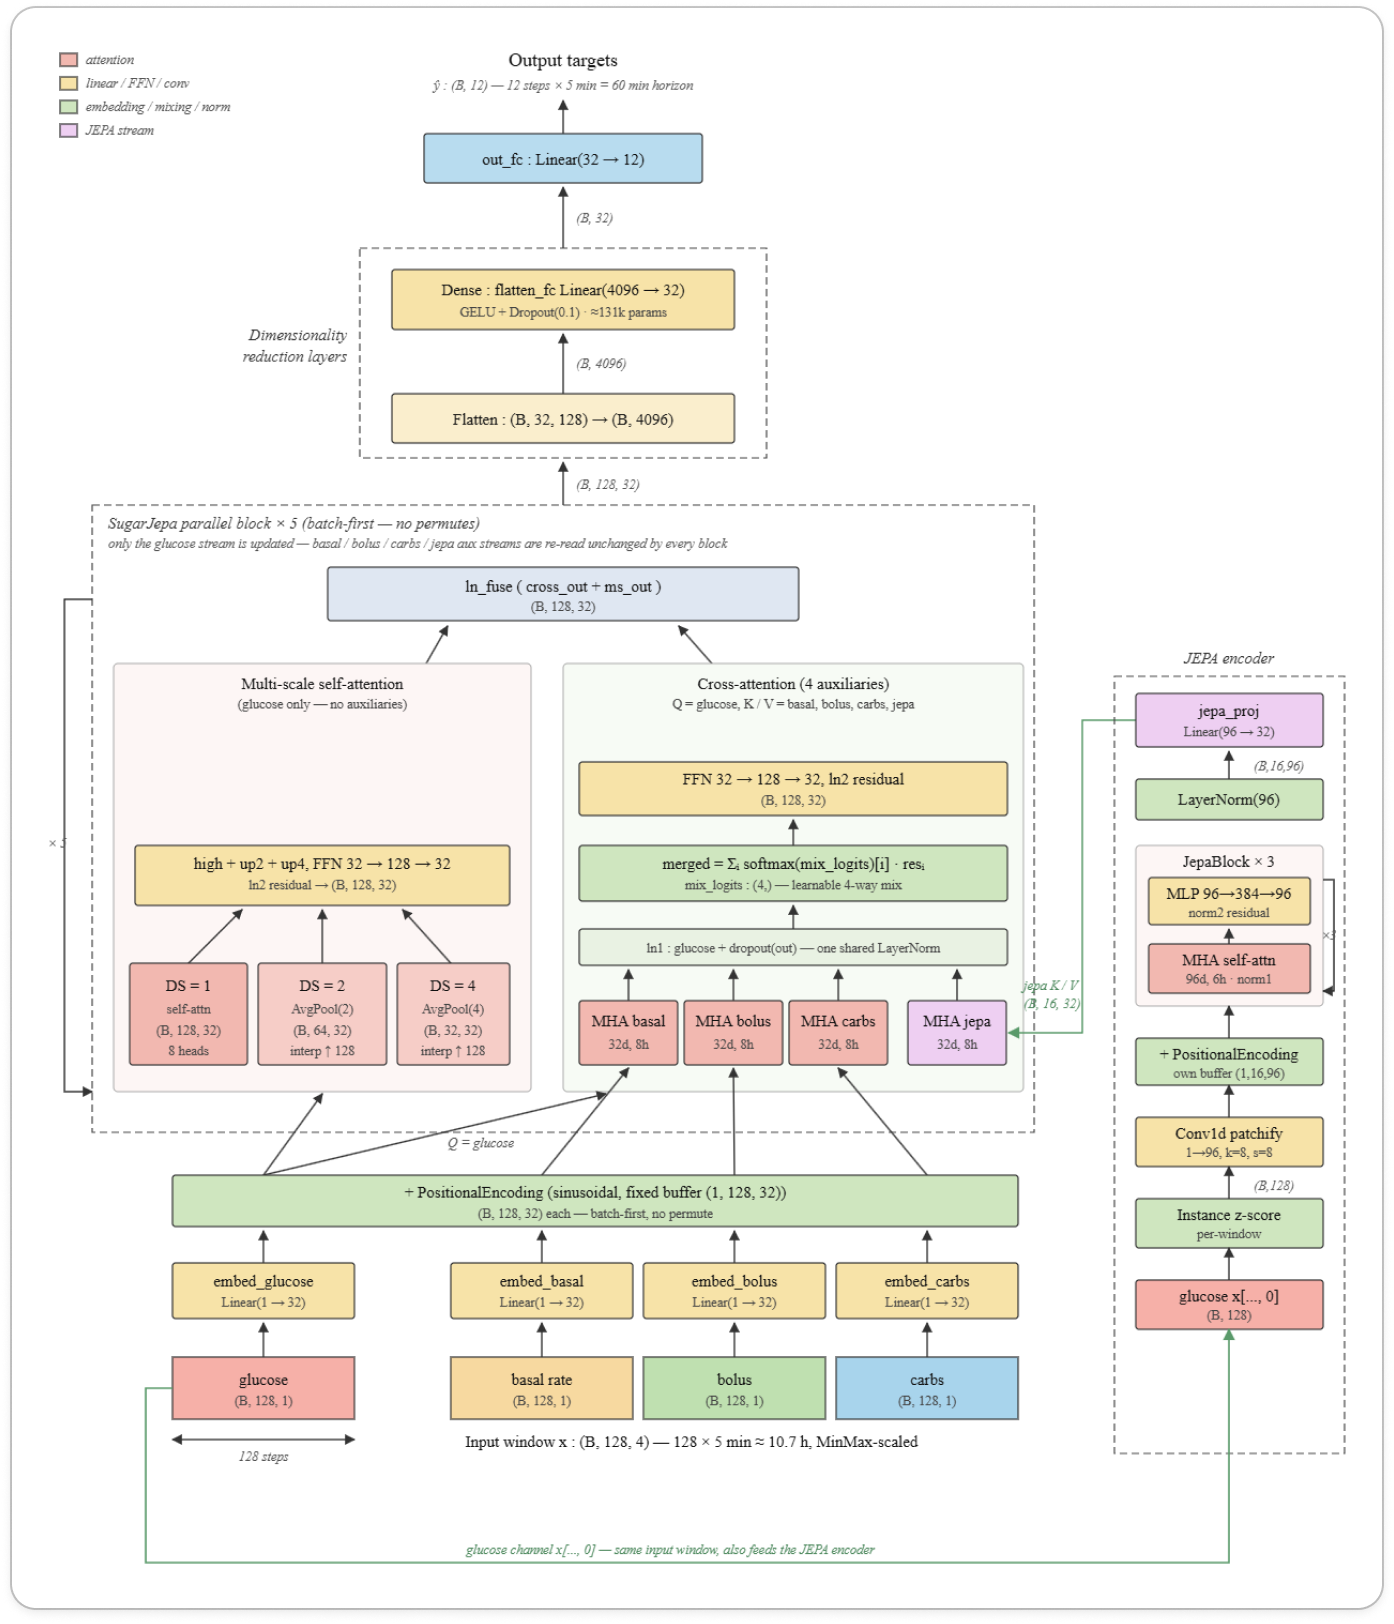
\includegraphics[width=0.8\textwidth]{sugar_jepa.png}
%     \caption{SugarJepa architecture. SugarOne with additional JEPA auxilary.}
%     \label{fig:model_architecture}
% \end{figure}

% In cases where encoder required input of $m$ points and SugarOne required $n$ points such that $m > n$, training windows were split to match $m$. Then, last $n$ points were used as input for SugarOne's main branches and the whole sequence was passed to JEPA. JEPA weights were not frozen, but had lower learning rate ($4 \cdot 10^{-5}$ vs $4 \cdot 10^{-4}$). Sugar One integration was evaluated with encoders \texttt{jepa-128-64}, \texttt{jepa-128}, \texttt{jepa-288}. For all cases, $n = 128$, and SugarOne was trained from scratch.

\section{Results}
\subsection{Encoder Evaluation}

To evaluate results of the encoder training we explored the generated latent space. 3-day encoder (\texttt{jepa-864}) showed the highest dimension utilization, and in general the number of actively used dimensions rose linearly with increase of the lookback window until collapsed for 7-day encoder (\texttt{jepa-2016}). Surprisingly, this effective rank collapse led to increase in mean std. Unlike all other encoders, this one displays highly unbalanced per-dimension std with few leading dimensions varying more than the rest (Table~\ref{tab:encoders_qc}, Figure~\ref{fig:jepa-encoders-qc}). 

\begin{table}[ht]
    \centering
    \begin{tabular}{lcc}
        \hline
        Encoder & effective rank & mean std \\
        \hline
        jepa-128-64 & 17.62 & 0.56 \\
        jepa-128 & 26.26 & 0.57 \\
        jepa-288 & 27.43 & 0.56 \\
        jepa-864 & \textbf{35.99} & 0.56 \\
        jepa-2016 & 16.71 & \textbf{0.83} \\
        \hline
    \end{tabular}
    \caption{QC metrics of the trained encoder. Effective rank shows how many of the dimensions are actively used for embedding generation. Mean std shows the average spread of the dimensions. Too low effective rank or std hint at the degenerate encoder that always outputs similar embeddings.}
    \label{tab:encoders_qc}
\end{table}

\begin{figure}[ht]
    \centering
    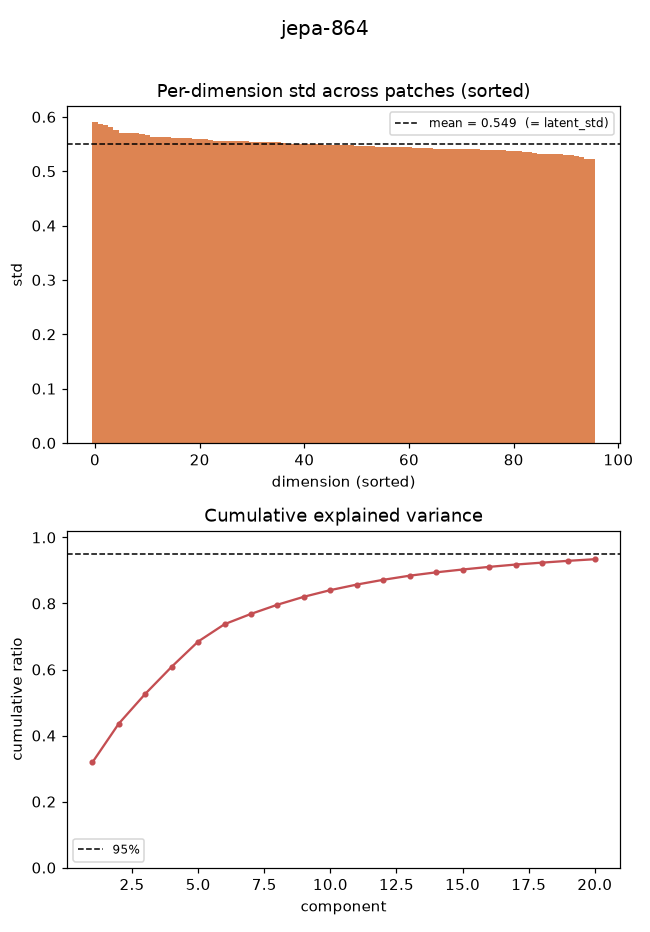
\includegraphics[width=0.48\textwidth]{jepa-864-encoder.png}
    \hfill
    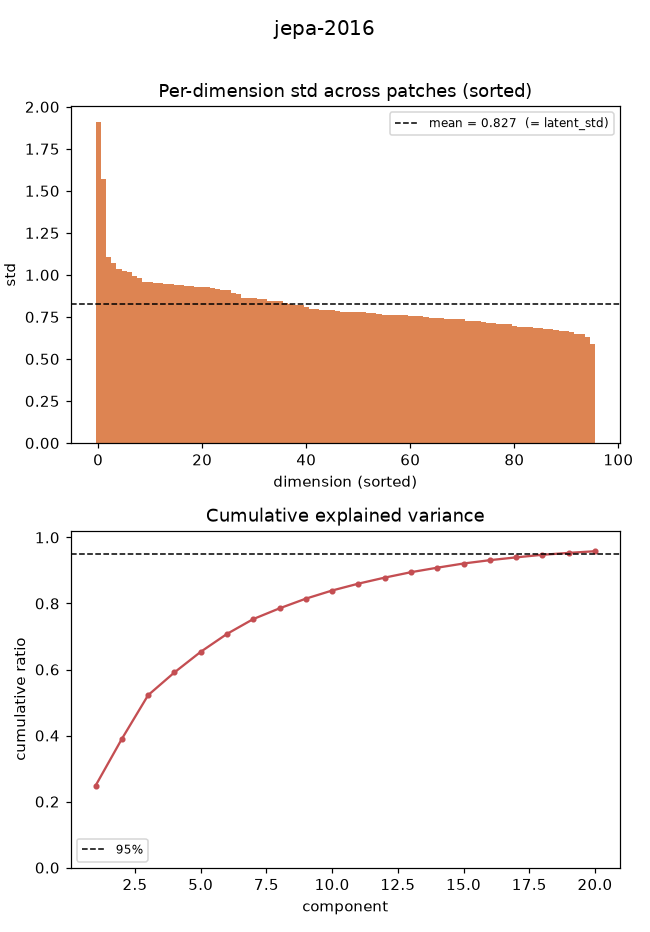
\includegraphics[width=0.48\textwidth]{jepa-2016-encoder.png}
    
    \caption{JEPA encoders comparison. 3-day encoder (left) shows higher effective rank and more even standard deviation across dimensions, while 7-day encoder (right) utilizes few dimensions that vary significantly more than the rest. PCA analyzis was performed on embeddings generated from withheld data. Lower plots show how individual PCs explain the variance of embeddings.}
    \label{fig:jepa-encoders-qc}
\end{figure}

% All encoder showed a strong ability to differentiate between the datasets used for training. Loop features much less users but much more per user sequences than AI READY. Based on  Figure~\ref{fig:jepa-864-pca} in all encoders PC1 was a good prediction of the dataset. The strongest separation was observed in the 3-day encoder, but it nevertheless remained healthy overall with silhouette coefficient for dataset remaining low (0.166), when all 96 dimensions were accounted (Figure~\ref{fig:jepa-864-pca}).

All encoders showed a strong ability to distinguish between the datasets used for training. The Loop dataset contains substantially fewer patients but many more sequences per patient than AI-READY. As illustrated in Figure~\ref{fig:jepa-864-pca}, the first principal component (PC1) provided a clear separation between the two datasets across all encoder variants. The strongest separation was observed for the 3-day encoder. Nevertheless, the overall representation remained well mixed, with a relatively low dataset-level silhouette coefficient of 0.166 when all 96 embedding dimensions were considered (Figure~\ref{fig:jepa-864-pca}).

\begin{figure}[ht]
    \centering
    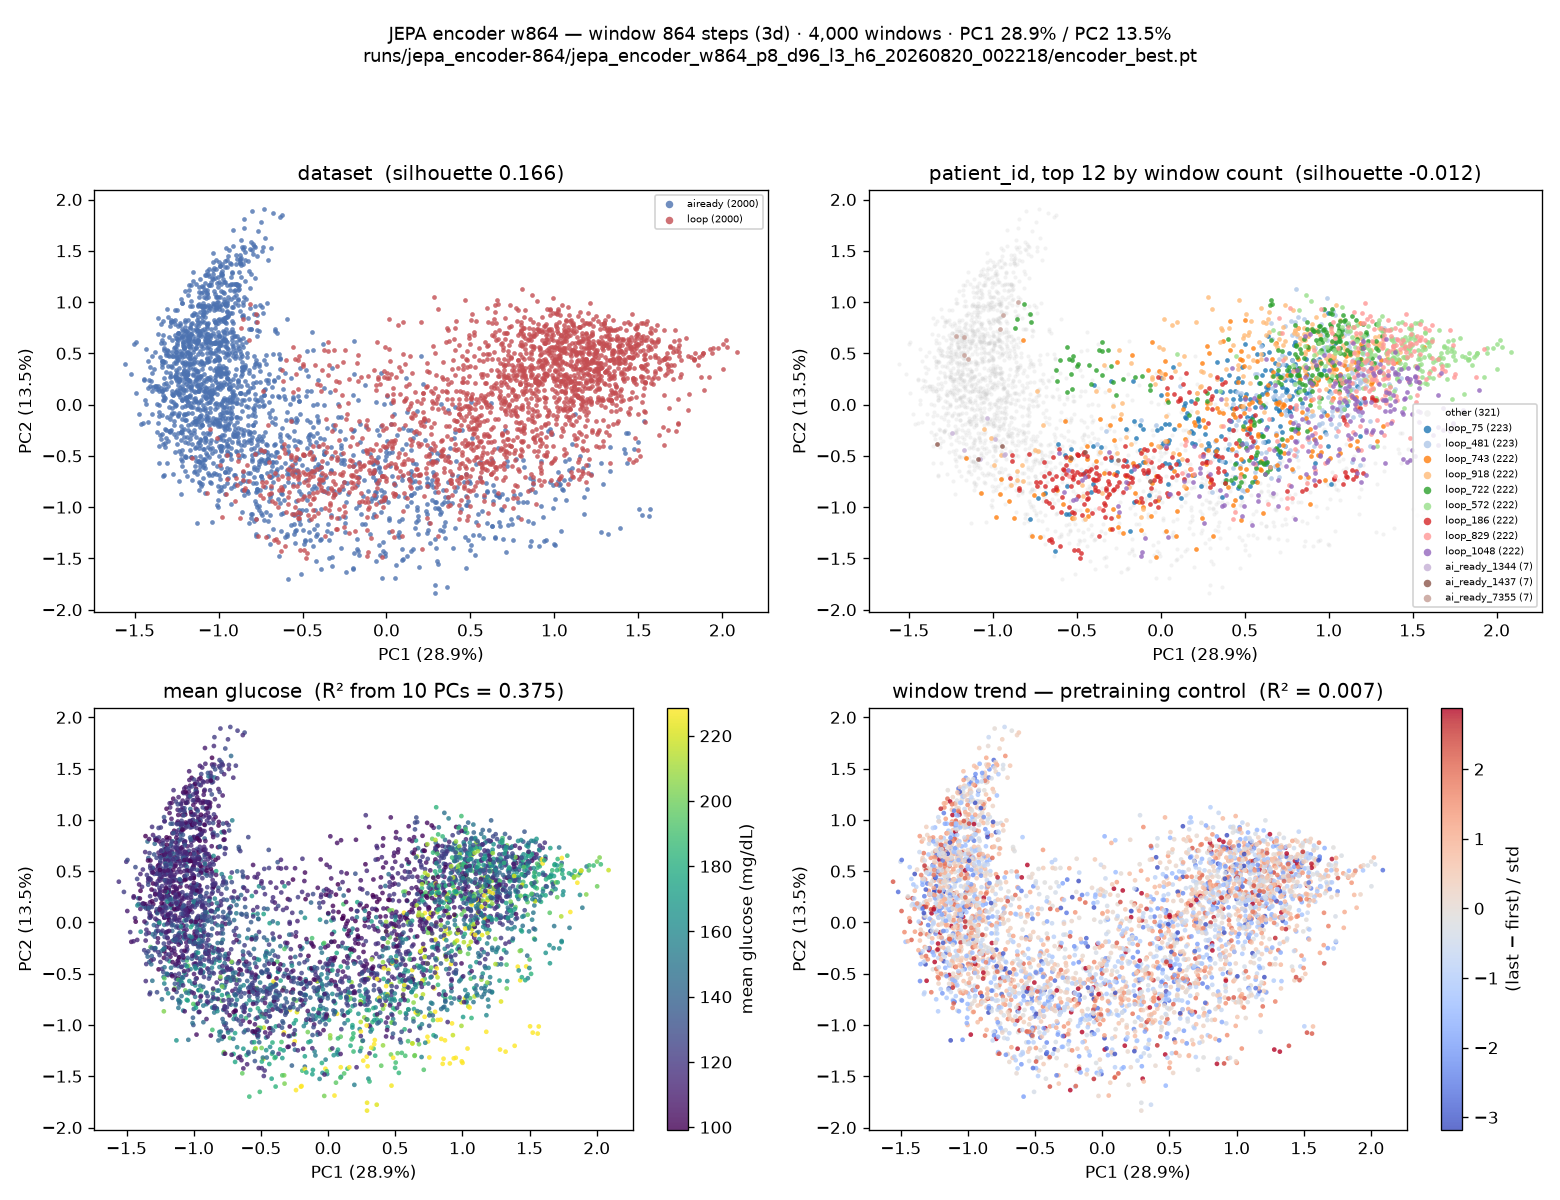
\includegraphics[width=0.8\textwidth]{pca_w864.png}
    
    \caption{jepa-864 Principal Component Analysis.}
    \label{fig:jepa-864-pca}
\end{figure}

\subsection{Patient identification from Jepa}

We performed linear probing on recovering patient id from the encoder, with a dense head trained on 300+, previously unseen, patients. Encoder's weights were frozen. 3-day encoder showed the best results in this test, reaching over 68\% accuracy on the validation split (Table~\ref{tab:jepa-patient-id-metrics}). Increase in window size seems to correlate with accuracy. For \texttt{jepa-2016} encoder it cannot be reliably evaluated though, as there are not enough (n = 18) patients with 7 consecutive days of glucose measurements.

% \begin{table}[ht]
%     \centering
%     \begin{tabular}{lcccc}
%         \hline
%         Encoder & Train Loss & Train Accuracy & Val Loss & Val Accuracy \\
%         \hline
%         jepa-128 & 4.0899 & 0.1362 & 4.4100 & 0.1132 \\
%         jepa-288 & 2.2380 & 0.4193 & 2.5915 & 0.3646 \\
%         \textbf{jepa-864} & \textbf{0.6864} & \textbf{0.8163} & \textbf{0.9636} & \textbf{0.6837} \\
%         jepa-2016 & 1.2329 & 0.5826 & 1.7063 & 0.4826 \\
%         \hline
%     \end{tabular}
%     \caption{JEPA encoder probing. Accuracy at recovering patient id (unseen patients) from frozen encoder's embeddings.}
%     \label{tab:jepa-patient-id-metrics}
% \end{table}

\begin{table}[ht]
    \centering
    \begin{tabular}{lcccc}
        \hline
        Encoder & Train Loss & Train Accuracy & Val Loss & Val Accuracy \\
        \hline
        jepa-128 & 4.0899 & 0.1362 & 4.4100 & 0.1132 \\
        jepa-288 & 2.2380 & 0.4193 & 2.5915 & 0.3646 \\
        \textbf{jepa-864} & \textbf{0.6864} & \textbf{0.8163} & \textbf{0.9636} & \textbf{0.6837} \\
        jepa-2016$^{*}$ & 1.2329 & 0.5826 & 1.7063 & 0.4826 \\
        \hline
    \end{tabular}
    \caption{JEPA encoder probing. Accuracy at recovering patient ID. $^{*}$The jepa-2016 model was evaluated on 18 patients, while all other models were evaluated on 665 patients.}
    \label{tab:jepa-patient-id-metrics}
\end{table}

\subsection{SugarJepa - Integrating JEPA into SugarOne}

Trained encoders were used as an auxiliary objective in SugarOne model, on par with bolus, carbs and basal. Overall, JEPA integration was beneficial, but the size of the encoder's input had a big influence on the gains. With 1-day encoder, frozen CGM-JEPA level of performance was reached with average MARD dropping to 9\% (threshold where the accuracy of prediction cannot be correctly evaluated due to the inherent sensor noise \citep{cgm-accuracy}) (Table~\ref{tab:sugar-jepa-test-metrics}). 3- and 7-day encoders pushed the metrics even lower, with \texttt{jepa-2016} variant scoring 8.10\% MARD (18\% improvement from the SugarOne baseline). At the same time, these gains are vanishing compared to the required increase in input data. For example, 3-day encoder achieved 14\% MARD improvement from the baseline (8.55) while requiring less than half of the data.  Per-study group metrics for every encoder can be found in (Table~\ref{tab:sugar-jepa-128-64-study-group-metrics}, Table~\ref{tab:sugar-jepa-128-study-group-metrics}, Table~\ref{tab:sugar-jepa-288-study-group-metrics}, Table~\ref{tab:sugar-jepa-864-study-group-metrics}, Table~\ref{tab:sugar-jepa-2016-study-group-metrics}, Table~\ref{tab:sugar-jepa-cgm-jepa-study-group-metrics}). In terms of encoder dimensionality, 96-dimension encoder showed better results than the 64-dimension one.

\begin{table}[ht]
    \centering
    \begin{tabular}{lccc}
        \hline
        Encoder & MAE & RMSE  & MARD \\
        \hline
        jepa-128-64 & 12.473596572875977 & 18.822355270385742 & 10.396651268005371 \\
        jepa-128 & 12.028145790100098 & 18.54257583618164 & 9.804486274719238 \\
        jepa-288 & 11.368544578552246 & 17.63058090209961 & 9.075223922729492 \\
        jepa-864 & 10.8974 & 17.0588 & 8.55 \\
        \textbf{jepa-2016} & \textbf{10.4014} & \textbf{16.1903} & \textbf{8.10} \\
        CGM-JEPA & 11.410141944885254 & 17.920860290527344 & 8.986237525939941 \\
        \hline
    \end{tabular}
    \caption{SugarJepa - test metrics}
    \label{tab:sugar-jepa-test-metrics}
\end{table}

\begin{table}[ht]
    \centering
    \begin{tabular}{lcccc}
        \hline
        Study Group & n windows & MAE & RMSE & MARD \\
        \hline
        Healthy & 213994 & 10.046438217163086 & 14.953590393066406 & 8.721386909484863 \\
        Pre-T2DM & 221588 & 10.309435844421387 & 15.539169311523438 & 8.445449829101562 \\
        Oral-T2DM & 223016 & 12.642668724060059 & 19.237953186035156 & 8.855355262756348 \\
        T1DM & 819013 & 13.377608299255371 & 19.932222366333008 & 12.199687957763672 \\
        Insulin-T2DM & 189826 & 13.637007713317871 & 20.715158462524414 & 8.594376564025879 \\
        \hline
    \end{tabular}
    \caption{SugarJepa (jepa-128-64 encoder) -- test metrics by study group}
    \label{tab:sugar-jepa-128-64-study-group-metrics}
\end{table}

\begin{table}[ht]
    \centering
    \begin{tabular}{lcccc}
        \hline
        Study Group & n windows & MAE & RMSE & MARD \\
        \hline
        Healthy & 213994 & 9.807256698608398 & 14.786678314208984 & 8.4523286819458 \\
        Pre-T2DM & 221588 & 10.099991798400879 & 15.407295227050781 & 8.207603454589844 \\
        Oral-T2DM & 223016 & 12.52254581451416 & 19.22431182861328 & 8.694753646850586 \\
        T1DM & 819013 & 12.670831680297852 & 19.463966369628906 & 11.23147964477539 \\
        Insulin-T2DM & 189826 & 13.428828239440918 & 20.68475341796875 & 8.339805603027344 \\
        \hline
    \end{tabular}
    \caption{SugarJepa (jepa-128 encoder) -- test metrics by study group}
    \label{tab:sugar-jepa-128-study-group-metrics}
\end{table}

\begin{table}[ht]
    \centering
    \begin{tabular}{lcccc}
        \hline
        Study Group & n windows & MAE & RMSE & MARD \\
        \hline
        Healthy & 194384 & 9.10853385925293 & 14.149213790893555 & 7.623103141784668 \\
        Pre-T2DM & 203055 & 9.530346870422363 & 14.836055755615234 & 7.555560111999512 \\
        T1DM & 702787 & 11.949230194091797 & 18.468379974365234 & 10.378556251525879 \\
        Oral-T2DM & 202258 & 12.080096244812012 & 18.471296310424805 & 8.284116744995117 \\
        Insulin-T2DM & 166952 & 12.929173469543457 & 19.644868850708008 & 8.086250305175781 \\
        \hline
    \end{tabular}
    \caption{SugarJepa (jepa-288 encoder) -- test metrics by study group}
    \label{tab:sugar-jepa-288-study-group-metrics}
\end{table}

\begin{table}[ht]
    \centering
    \begin{tabular}{lcccc}
        \hline
        Study Group & n windows & MAE & RMSE & MARD \\
        \hline
        Healthy & 136231 & 8.794051170349121 & 13.750545501708984 & 7.211543560028076 \\
        Pre-T2DM & 145715 & 9.272398948669434 & 14.495078086853027 & 7.27789831161499 \\
        T1DM & 432333 & 11.484896659851074 & 17.918399810791016 & 9.818462371826172 \\
        Oral-T2DM & 142733 & 11.598993301391602 & 17.956985473632812 & 7.8462748527526855 \\
        Insulin-T2DM & 110509 & 12.428182601928711 & 19.106578826904297 & 7.847798824310303 \\
        \hline
    \end{tabular}
    \caption{SugarJepa (jepa-864 encoder) -- test metrics by study group}
    \label{tab:sugar-jepa-864-study-group-metrics}
\end{table}

\begin{table}[ht]
    \centering
    \begin{tabular}{lcccc}
        \hline
        Study Group & n windows & MAE & RMSE & MARD \\
        \hline
        Healthy & 49201 & 8.4966 & 13.2878 & 6.85 \\
        Pre-T2DM & 50893 & 9.1485 & 14.2153 & 7.28 \\
        T1DM & 111812 & 10.8211 & 16.7306 & 9.31 \\
        Oral-T2DM & 48076 & 11.3357 & 17.4954 & 7.61 \\
        Insulin-T2DM & 35951 & 12.2269 & 18.7117 & 7.89 \\
        \hline
    \end{tabular}
    \caption{SugarJepa (jepa-2016 encoder) -- test metrics by study group}
    \label{tab:sugar-jepa-2016-study-group-metrics}
\end{table}

\begin{table}[ht]
    \centering
    \begin{tabular}{lcccc}
        \hline
        Study Group & n windows & MAE & RMSE & MARD \\
        \hline
        Healthy & 194384 & 9.149588584899902 & 14.270050048828125 & 7.57526159286499 \\
        Pre-T2DM & 203055 & 9.544251441955566 & 14.909406661987305 & 7.486485004425049 \\
        Oral-T2DM & 202258 & 11.951461791992188 & 18.540788650512695 & 8.105234146118164 \\
        T1DM & 702787 & 12.059324264526367 & 18.895479202270508 & 10.304533004760742 \\
        Insulin-T2DM & 166952 & 12.922983169555664 & 19.995197296142578 & 7.971052646636963 \\
        \hline
    \end{tabular}
    \caption{SugarJepa (CGM-JEPA encoder) -- test metrics by study group}
    \label{tab:sugar-jepa-cgm-jepa-study-group-metrics}
\end{table}

\subsection{SugarJepa finetuning}

We then tested performance of SugarJepa model on a holdout set of Loop users and a personal dataset provided by a co-author (Author1). We recorded zero-shot performance as well as fine-tuned performance. During fine-tuning, JEPA encoder remained frozen and only the main model's weight was updated. All models started from \texttt{jepa-288} beat SugarOne baseline on zero-shot, in most cases outperforming even fine-tuned version on horizon of 30-60 days. For zero-shot, dependency between the encoder's context size and improvement was linear in all cases except of Author1's data where \texttt{jepa-288} showed the best result (17.64). Fine-tuning benefited 1- and 3-day encoders most, with their performance beating that of the \texttt{jepa-2016}, which in most cases regressed from fine-tuning. With that said, fine-tuned versions surpassed their own zero-shot MAE but often struggled to reach the level of zero-shot \texttt{jepa-2016}. Given that in many cases there were not enough data for the 7 consecutive days of glucose we propose to use \texttt{jepa-288} and \texttt{jepa-864} as the models most suitable to practical use. Fine-tuning was not performed for cases where there was not enough data to train and evaluate the model correctly. 

\begin{tabular}{lcccccccc}
  \hline
  Model & Zero-shot & 1d & 3d & 7d & 14d & 30d & 60d & All \\
  \hline
  \multicolumn{9}{l}{\textit{Author1}} \\
  SugarOne & 18.31 & 18.42 & 18.60 & 18.88 & 18.48 & 18.06 & 17.54 & 16.98 \\
  jepa-128-64 & 18.05 & 19.14 & 17.56 & 17.30 & 17.26 & 17.31 & 16.90 & 16.76 \\
  jepa-128 & 17.67 & \textbf{18.10} & \textbf{17.55} & 17.24 & 17.24 & 17.20 & 16.95 & 16.69 \\
  jepa-288 & \textbf{17.64} & -- & 17.61 & \textbf{17.21} & \textbf{17.09} & \textbf{17.12} & \textbf{16.83} & \textbf{16.53} \\
  jepa-864 & 17.97 & -- & -- & 17.91 & 17.69 & 17.96 & 17.42 & 16.69 \\
  jepa-2016 & 18.61 & -- & -- & -- & 18.07 & 18.15 & 17.46 & 17.79 \\
  \hline
  \multicolumn{9}{l}{\textit{Loop 154}} \\
  SugarOne & 24.61 & \textbf{24.74} & 24.57 & 24.57 & 24.57 & 24.84 & 24.81 & 24.12 \\
  jepa-128-64 & 25.40 & 24.89 & 24.30 & 24.30 & 24.30 & 24.47 & 24.01 & 23.64 \\
  jepa-128 & 25.48 & 25.22 & 24.59 & 24.59 & 24.59 & 24.67 & 24.33 & 23.90 \\
  jepa-288 & 23.13 & -- & \textbf{22.84} & \textbf{22.84} & \textbf{22.84} & \textbf{22.82} & \textbf{22.87} & 22.66 \\
  jepa-864 & 22.74 & -- & -- & -- & -- & -- & -- & \textbf{22.58} \\
  jepa-2016 & \textbf{21.93} & -- & -- & -- & -- & -- & -- & 27.28 \\
  \hline
  \multicolumn{9}{l}{\textit{Loop 556}} \\
  SugarOne & 18.10 & 17.74 & 18.00 & 17.89 & 18.40 & 17.65 & 17.25 & 17.39 \\
  jepa-128-64 & 17.52 & \textbf{17.47} & 17.40 & 17.36 & 17.50 & 17.19 & 16.90 & 16.92 \\
  jepa-128 & 17.46 & 17.79 & 17.52 & 17.55 & 17.64 & 17.61 & 17.25 & 17.01 \\
  jepa-288 & 17.22 & -- & \textbf{16.94} & 16.94 & 16.96 & 17.11 & 17.03 & 16.65 \\
  jepa-864 & 16.46 & -- & -- & \textbf{16.38} & \textbf{16.62} & 16.52 & 16.60 & 16.00 \\
  jepa-2016 & \textbf{15.30} & -- & -- & -- & 19.69 & \textbf{15.18} & \textbf{15.49} & \textbf{15.49} \\
  \hline
  \multicolumn{9}{l}{\textit{Loop 730}} \\
  SugarOne & 18.06 & 18.27 & 18.42 & 18.31 & 18.02 & 18.23 & 16.52 & 16.50 \\
  jepa-128-64 & 16.35 & \textbf{16.43} & 16.50 & 16.24 & 16.23 & 16.39 & 16.13 & 16.06 \\
  jepa-128 & 16.36 & 16.44 & 16.46 & 16.24 & 16.31 & 16.47 & 16.24 & 16.14 \\
  jepa-288 & 16.02 & -- & \textbf{15.90} & \textbf{15.92} & 15.80 & 15.73 & \textbf{15.71} & 15.62 \\
  jepa-864 & 16.17 & -- & -- & 16.05 & 16.05 & 16.04 & 15.91 & 15.83 \\
  jepa-2016 & \textbf{14.73} & -- & -- & -- & \textbf{14.95} & \textbf{14.93} & 15.75 & \textbf{15.39} \\
  \hline
  \multicolumn{9}{l}{\textit{Loop 1017}} \\
  SugarOne & 17.69 & 17.85 & 17.89 & 17.91 & 18.01 & 18.30 & 17.38 & 16.95 \\
  jepa-128-64 & 18.20 & 17.88 & 17.95 & 17.96 & 17.93 & 17.72 & 16.89 & 16.62 \\
  jepa-128 & 17.97 & \textbf{17.81} & 17.80 & 17.78 & 17.88 & 17.63 & 17.00 & 16.75 \\
  jepa-288 & 17.41 & -- & \textbf{17.37} & \textbf{17.37} & \textbf{16.93} & 16.94 & \textbf{16.58} & \textbf{16.38} \\
  jepa-864 & \textbf{16.62} & -- & -- & -- & -- & \textbf{16.85} & 17.01 & 16.83 \\
  jepa-2016 & -- & -- & -- & -- & -- & -- & -- & -- \\
  \hline
  \multicolumn{9}{l}{\textit{Loop 1029}} \\
  SugarOne & 22.62 & 22.66 & 22.67 & 22.68 & 22.22 & 22.81 & 21.04 & 20.94 \\
  jepa-128-64 & 20.93 & 20.97 & 20.88 & 20.49 & 20.57 & 20.40 & 19.96 & 19.90 \\
  jepa-128 & 20.60 & \textbf{20.81} & 20.56 & 20.41 & \textbf{20.36} & 20.24 & 20.04 & 20.01 \\
  jepa-288 & 20.30 & -- & \textbf{20.28} & \textbf{20.28} & 20.78 & \textbf{19.94} & \textbf{19.52} & 19.55 \\
  jepa-864 & \textbf{19.37} & -- & -- & -- & -- & -- & 20.38 & \textbf{19.45} \\
  jepa-2016 & 24.22 & -- & -- & -- & -- & -- & -- & 22.91 \\
  \hline
  \multicolumn{9}{l}{\textit{Loop 1082}} \\
  SugarOne & 17.00 & 16.97 & 17.08 & 17.13 & 17.20 & 17.60 & -- & 17.79 \\
  jepa-128-64 & 16.54 & 16.55 & 16.55 & 16.36 & 16.41 & 16.56 & -- & 16.65 \\
  jepa-128 & 16.57 & \textbf{16.54} & 16.54 & 16.48 & 16.51 & 16.62 & -- & 16.66 \\
  jepa-288 & 15.17 & -- & \textbf{15.59} & 15.36 & 15.04 & 15.10 & -- & 15.19 \\
  jepa-864 & \textbf{14.78} & -- & -- & \textbf{14.83} & \textbf{14.97} & \textbf{14.97} & -- & \textbf{14.97} \\
  jepa-2016 & -- & -- & -- & -- & -- & -- & -- & -- \\
  \hline
  \multicolumn{9}{l}{\textit{Mean}} \\
  SugarOne & 19.48 & 19.52 & 19.61 & 19.62 & 19.56 & 19.64 & 19.09 & 18.67 \\
  jepa-128-64 & 19.00 & 19.05 & 18.74 & 18.57 & 18.60 & 18.58 & 18.47 & 18.08 \\
  jepa-128 & 18.87 & \textbf{18.96} & 18.72 & 18.61 & 18.65 & 18.63 & 18.64 & 18.16 \\
  jepa-288 & 18.13 & -- & \textbf{18.08} & 17.99 & 17.92 & 17.82 & 18.09 & 17.51 \\
  jepa-864 & \textbf{17.73} & -- & -- & \textbf{16.29} & \textbf{16.33} & 16.47 & 17.46 & \textbf{17.48} \\
  jepa-2016 & 18.96 & -- & -- & -- & 17.57 & \textbf{16.09} & \textbf{16.23} & 19.77 \\
  \hline
  \caption{SugarJepa finetuning results.}
    \label{tab:sugar-jepa-finetuning}
\end{tabular}

\section{Discussion}
We show that incorporating JEPA approach into a glucose forecasting pipeline as an additional objective is beneficial and provides up to 15-18\% improvement across typical metrics. The encoder can also be used for patient embedding generation, enabling individual patient recognition with up to 68\% accuracy. Quality of JEPA representation benefits from increasing the look-back window, but the effect vanishes for glucose prediction task and reverses after the optimal point of 3 days. Subsequent improvements in glucose forecasting seem to be possible in theory, but are limited by the inherent CGM reading noise. Utilizing 3-day encoder seems optimal to the task, as it requires the modest amount of data while providing substantial benefits over the baseline SugarOne model and shorter window encoders.

Fine-tuning comparison showed that JEPA-embedded models outperform the SugarOne even when the former work in zero-shot mode and the latter is fine-tuned on 30+ days of personalized glucose measurements. Further fine-tuning of SugarJepa model futher improved the results.

One limitation of the study is that incorporating JEPA should be beneficial for cross-modal tasks. In case of glucose forecasting that could be forecast on blood vs GCM data using the same encoder, as shown in \cite{muhammad2026cgm}. We did not evaluate SugarOne or SugarJepa models on blood glucose measurements, aiming specifically for GCM devices.

Another limitation is that better methods for self-supervised encoder training could be available, e.g. Sketched Isotropic Gaussian Regularization (SigReg) \cite{lecun2026lejepa}. We intend to incorporate them in our work as the next steps.

\section{Conclusion}
Summarise your contribution in a few sentences.

% --- References ----------------------------------------------
% References and any appendix do NOT count toward the 8-page limit.
% \bibliographystyle{plainnat}
% \bibliography{references}
% \begin{thebibliography}{99}
% \bibitem{vicreg}
% Bardes, A., Ponce, J., \& LeCun, Y. (2022). VICReg: Variance-Invariance-Covariance Regularization for Self-Supervised Learning (arXiv:2105.04906). arXiv. https://doi.org/10.48550/arXiv.2105.04906 
% \bibitem{cgm-accuracy}
% Garg, S. K., Kipnes, M., Castorino, K., Bailey, T. S., Akturk, H. K., Welsh, J. B., Christiansen, M. P., Balo, A. K., Brown, S. A., Reid, J. L., \& Beck, S. E. (2022). Accuracy and Safety of Dexcom G7 Continuous Glucose Monitoring in Adults with Diabetes. Diabetes Technology \& Therapeutics, 24(6), 373–380. https://doi.org/10.1089/dia.2022.0011 
% \end{thebibliography}

% --- References ----------------------------------------------
% References and any appendix do NOT count toward the 8-page limit.
\bibliographystyle{plainnat}
\bibliography{references}

% --- Appendix (optional; does NOT count toward the limit) ----
\appendix
\section{Appendix}
Supplementary material, proofs, or extra detail may go here.

\end{document}